% !TEX root = ../notes_template.tex

\chapter{테일러 급수와 로랑 급수}

이 장에서는 영역 $D$에 정의된 복소해석함수 $f$는 
$D$의 임의의 점에서 급수 전개가 가능하다는 근본적인 성질을 먼저 공부할 것이다.
다음 그림에서 왼쪽을 참고하라.
\begin{figure*}[h!]
\begin{center}
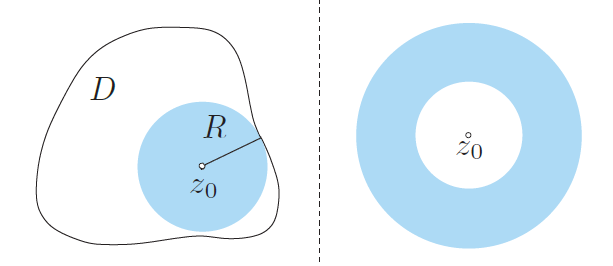
\includegraphics[width=0.5\textwidth]{./SaltChapter/fig-4-0-1}
\end{center}
\end{figure*}
\[
\text{테일러 급수: } \sum_{n=0}^\infty c_n(z-z_0)^n 
\quad
\text{로랑 급수: } \sum_{n\in \mathbb Z} c_n(z-z_0)^n 
\]

즉, 각각의 $z_0 \in D$에 대하여 다음을 만족하는 $R>0$이 존재한다.
\[
f(z) = \sum_{n=0}^\infty c_n(z-z_0)^n, \quad |z-z_0| <R.
\]
역으로,  적당한 $R$에 대하여 $|z-z_0|<R$을 만족하는 두 개 이상의 점에서 급수
\[
\sum_{n=0}^\infty c_n(z-z_0)^n
\]
가 수렴하면 $|z-z_0|<R$에서 복소해석함수이다.
이를 보이는 과정에서 복소해석함수에 대한 근본적인 성질들을 증명할 것이다.
\begin{itemize}
\item[(1)] (일반화된) 코시 적분공식과 코시 부등식
\item[(2)] 해의 분류와 항등정리
\item[(3)] 최대절대값정리
\end{itemize}

이 장의 후반부에서는
급수와 유사하지만 $z-z_0$ 항의 지수를 음의 정수까지 확장한
로랑 급수를 공부할 것이다.
이는 원환(특히 뚫린 원판)에 정의된 복소해석함수를 연구하는데 특히 유용하다,
앞의 그림에서 오른쪽을 참고하라.
끝으로 로랑 급수는 ``특이점''의 분류와 실함수 적분의 계산에도 유용함을 살펴볼 것이다.

\section{급수}

실수열의 경우와 유사하게 주어진
복소수열 $(a_n)_{n\in\mathbb N}$에 대하여
부분합 수열 $(s_n)_{n\in\mathbb N}$을 만들 수 있다.
\begin{align*}
s_1 &:= a_1, \\
s_2 &:= a_1 + a_2, \\
s_3 &:= a_1 + a_2 + a_3, \\
& \vdots
\end{align*}

\begin{salt_definition} \label{def-4-1}
\
\begin{itemize}
\item[(1)] 복소수열 $(s_n)_{n\in\mathbb N}$이 수렴하면
$\sum\limits_{n=1}^\infty a_n := \lim\limits_{n\to\infty} s_n$라 쓰고
급수 $\sum\limits_{n=1}^\infty a_n$이 {\bf 수렴한다}고 정의한다.
\item[(2)] 복소수열 $(s_n)_{n\in\mathbb N}$이 발산하면,
급수 $\sum\limits_{n=1}^\infty a_n$는 {\bf 발산한다}고 정의한다.
\item[(3)] 실급수 $\sum\limits_{n=1}^\infty |a_n|$이 수렴하면,
급수 $\sum\limits_{n=1}^\infty a_n$은 {\bf 절대수렴한다}고 정의한다.
\end{itemize}
\end{salt_definition}

복소수열이 수렴할 필요충분조건은
실수부와 허수부로 만든 수열이 각각 수렴하는 것이라는 
연습문제 \ref{ex-1-25}의 결과로부터,
\[
\sum\limits_{n=1}^\infty a_n\,\text{이 수렴한다. }
\Longleftrightarrow \text{\textcolor{red}{ 실수열} }
\sum\limits_{n=1}^\infty \Re(a_n)\, \text{과 }
\sum\limits_{n=1}^\infty \Im(a_n)\,\text{가 수렴한다.}
\]
따라서  실해석학의 결과를 아용하여 복소수열의 수렴성을 판정할 수 있다.
예를 들면, 다음 결과들을 쉽게 얻을 수 있는데 이는 연습문제로 남긴다.

\begin{salt_exercise}\label{ex-4-1}
$\Sum_{n=1}^\infty a_n$이 수렴하면, $\Lim_{n\to\infty}a_n = 0$임을 보여라.
\end{salt_exercise}

\begin{salt_exercise}\label{ex-4-2}
$\Sum_{n=1}^\infty a_n$이 절대수렴하면, $\Sum_{n=1}^\infty a_n$이 수렴함을 증명하라.
\end{salt_exercise}

\begin{salt_exercise}\label{ex-4-3}
$|z|<1$이면 $\Sum_{n=0}^\infty z^n$이 수렴하고 
$\Sum_{n=0}^\infty z^n = \dfrac1{1-z}$임을 보여라.
\end{salt_exercise}

\begin{salt_exercise}\label{ex-4-4}
$|z|<1$이면 $\Sum_{n=0}^\infty nz^{(n-1)^2}$임을 보여라.
\end{salt_exercise}

\begin{salt_exercise}\label{ex-4-5}
$\Re(s)>0$인 모든 복소수 $s\in \mathbb C$에 대하여
$1^{-s} +  2^{-s} + 3^{-s} + \cdots$가 수렴함을 보여라.
그러면
\[
s \mapsto \zeta(s) := \sum_{n=1}^\infty \dfrac1{n^s}
\]
\end{salt_exercise}
는 반평면 $\Re(s)>1$에서 잘 정의된 함수가 되며, 이를 
{\bf 리만 제타함수}라고 한다.
리만 제타함수와 정수론의 소수이론을 연결한 {\bf 오일러 곱셈공식}에 따르면,
소수를 증가하는 순서대로 나열한
$p_1:=2 < p_2:=3 < p_3:=5 < \cdots$를 무한 소수열로 정의할 때 다음이 성립한다.
\[
\zeta(s) = \lim_{K\to \infty} \prod_{k=1}^K \dfrac1{1-p_k^{-s}},
\quad \Re(s)>1.
\]
버나드 리만(1826-1866)은 제타함수 $\zeta$를 확장하여 $\mathbb C\setminus \{1\}$의 
복소해석함수로 정의할 수 있음을 보였다. 
$\zeta$는 $-2, -4, -6, \ldots$에서 ``자명해(trivial zero)''를 갖지면
다른 해도 존재한다. 리만이 계산한 모든 비자명해(nontrivial zero)는 모두 직선 $\Re(s) = 1/2$위에
있다. 이로부터 리만은 다음과 같이 예측(conjecture)하였는데 이는 여전히 수학계의 유명한 미해결 문제이다.

\begin{salt_conjecture}[리만가설] \label{conj-4-1}
리만 제타함수의 모든 비자명해는 직선 $\Re(s) = 1/2$ 위에 있다.
\end{salt_conjecture}

\section{급수}

\subsection{제곱급수와 수렴영역}

$(c_n)_{n\in\mathbb N}$을 복소수열이라고 하자.
다음과 같은 표현을
\[
\sum_{n=0}^\infty c_nz^n
\]
복소수 변수 $z$의 제곱급수라고 한다 ($(c_n)_{n\in\mathbb N}$을 계수들의 수열로 생각해도 된다).
이제 특정한 값을 급수의  $z$에 대입하는 경우를 생각해볼 수 있다.
그러면 어떤 $z\in\mathbb C$에 대하여 제곱급수가 수렴할 수 있고, 
다른 값에서는 발산할 수도 있다.

\begin{salt_example}\label{example-4-1}
모든 다항식은 유한개의 항에서만 계수가 $0$이 아닌 제곱급수 꼴로 쓸 수 있다.
따라서 다항식은 모든 $z\in\mathbb C$에 대하여 수렴한다.

제곱급수  
\[
\sum_{n=0}^\infty z^n
\]
는 $|z|<1$에서 수렴한다. 
$|z|\ge1$에서 급수는 발산한다 (왜냐하면 $\Lim_{n\to\infty} z^n = 0$이 성립하지 않으므로).
\hfill$\diamondsuit$
\end{salt_example}

근본적인 질문으로 
\begin{center}
어떤 $z\in\mathbb C$에 대하여  급수 $\sum_{n=0}^\infty c_nz^n$가 수렴하는가?
\end{center}

이 문제에 대한 답은 다음 정리에서 얻을 수 있다.

\begin{salt_theorem} \label{thm-4-1}
제곱급수 $\Sum_{n=0}^\infty c_nz^n$에 대하여
다음 두 가지 중 정확히 하나만 성립한다.
\begin{itemize}
\item[(1)] 모든 $z\in\mathbb C$에 대하여 절대수렴하거나
\item[(2)] 음이 아닌 실수 $R$이 유일하게 존재하여 다음을 만족한다.
\begin{itemize}
\item[(a)] $|z|<R$인 모든 $z\in\mathbb C$에 대하여 $\Sum_{n=0}^\infty c_nz^n$이 절대수렴하고,
\item[(b)] $|z|>R$인 모든 $z\in\mathbb C$에 대하여 $\Sum_{n=0}^\infty c_nz^n$는 발산한다.
\end{itemize}
\end{itemize}
\end{salt_theorem}

위 정리에서 유일한 $R>0$을 급수의 수렴반경이라 부른다.
급수가 모든 $z\in\mathbb C$에 대하여 수렴하면
무한대의 수렴반경을 가지며 ``$R=\infty$''라 쓴다.

\begin{figure}[h!]
\begin{center}
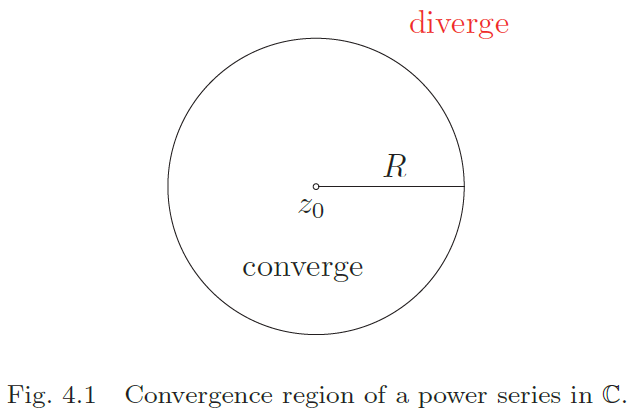
\includegraphics[width=0.5\textwidth]{./SaltChapter/fig-4-1}
\end{center}
\caption{$\mathbb C$에 정의된 제곱급수의 수렴영역}
\label{fig-4-1}
\end{figure}

원 $|z|=R$에서는 어떻게 될까?
복소 제곱급수는 $|z|=R$로 주어진 경계의 모든 점에서 발산하거나,
어떤 점에서는 발산하고 어떤 점에서는 수렴하거나,
아니면 경계의 모든 점에서 수렴할 수도 있다.
경계위의 각 점에 대하여 어떻게 되는지 답을 구하는 일반적인 방법은 없다.
특정한 제곱급수가 주어지면 그 특성에 따라 찾아 직접 확인해야 한다,

{\bf 증명} (정리 \ref{thm-4-1})

\[
S:= \left\{ y\in [0,\infty) \,:\,
\exists z\in \mathbb C, y=|z| \text{ 이고 } \Sum_{n=0}^\infty c_nz^n \text{이 수렴한다.}
\right\}
\]
라 정의하자.
$0\in S$은 분명하기에 $S$는 공집합이 아니며
다음 두 가지 경우가 가능하다.

$\underline{1}^\circ$ $S$가 위로 유계가 아닌 경우:
이 경우는 수렴반경은 무한대가 됨을 보일 것이다.
$z\in \mathbb C$가 주어졌다고 하면,
$|z|<y$인 $y\in S$가 존재한다.
 그런데 $y\in S$이므로 $y=|z_0|$이고
\[
\sum_{n=0}^\infty c_n z_0^n
\]
이 수렴하는 $z_0\in S$가 존재한다.
이로부터 $n\to\infty$일 때 각 항이 $0$으로 수렴한다.
특히, 각 항은  $|c_nz_0^n| \le M$으로 유계이다.
이제 $r:=|z|/|z_0| (<1)$로 잡으면
\[
|c_nz^n| = |c_nz_0^n| \left( \dfrac{|z|}{|z_0|}\right)^n
\le Mr^n \quad (n\in \mathbb N).
\]
한편 $\sum\limits_{n=0}^\infty Mr^n$이 수렴한다 ($r<1$).
비교판정법을 쓰면 
\[
\sum_{n=0}^\infty c_n z^n
\]
은 절대수렴한다. $z$는 우리가 임의로 선택할 수 있기 때문에
정리의 (1)이 성립한다,


$\underline{2}^\circ$ $S$가 위로 유계인 경우:
이 경우 수렴반경이 $\sup S$가 됨을 보일 것이다.
즉,
\begin{itemize}
\item[(a)] $|z|<\sup S$이면
$\Sum_{n=0}^\infty c_nz^n$이 절대수렴하고,
\item[(b)] $|z|>\sup S$이면  $\Sum_{n=0}^\infty c_nz^n$는 발산한다.
\end{itemize}
$z\in S$가 $|z|<\sup S$를 만족하면
상한(supremum)의 %= ##[SALT] 용어확인
정의에 따라,
$|z|<y$인 $y\in S$가 존재한다. 
그러면 $\underline{1}^\circ$ $S$의 증명과정을 아래와 같이 반복할 수 있다.
$y\in S$이므로
$y=|z_0|$이고
\[
\sum_{n=0}^\infty c_n z_0^n
\]
이 수렴하는 $z_0\in S$가 존재한다.
이로부터 $n\to\infty$일 때 각 항이 $0$으로 수렴한다.
특히, 각 항은 $|c_nz_0^n| \le M$으로 유계이다.
이제 $r:=|z|/|z_0| (<1)$로 잡으면
\[
|c_nz^n| = |c_nz_0^n| \left( \dfrac{|z|}{|z_0|}\right)^n
\le Mr^n \quad (n\in \mathbb N).
\]
한편 $\sum\limits_{n=0}^\infty Mr^n$이 수렴한다 ($r<1$).
비교판정법을 쓰면 
\[
\sum_{n=0}^\infty c_n z^n
\]
은 절대수렴한다.
끝으로, $z\in \mathbb C$가 $|z|>\sup S$를 만족하면,
$y:=|z|$라 할 때
$y \in S$이고 $S$의 정의로부터 
\[
\sum_{n=0}^\infty c_n z^n
\]
이 발산한다 (그렇지 않다면 $y\in S$를 만족해야 한다).

\begin{figure*}[h!]
\begin{center}
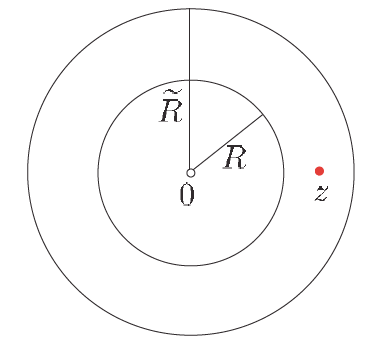
\includegraphics[width=0.3\textwidth]{./SaltChapter/fig-4-0-2}
\end{center}
%\caption{$\mathbb C$에 정의된 제곱급수의 수렴영역}
%\label{fig-4-1}
\end{figure*}

$R$의 유일성은 다음과 같이 증명된다.
$R$과 $\tilde R$이 정리의 조건을 만족하고 $R<\tilde R$이라 하자.
그러면
\[
R < r:= \dfrac{R+\tilde R}{2} < \tilde R.
\]
$r<\tilde R$로부터
$\Sum_{n=0}^\infty c_n r^n$이 수렴하고,
$R<r$로부터 $\Sum_{n=0}^\infty c_n r^n$은 발산하며
모순이 된다.
\hfill $\square$

다음 결과를 이용하면
몇가지 경우의 수렴반경를 계산할 수 있다,

 \begin{salt_theorem} \label{thm-4-2}
제곱급수 
\[
\Sum_{n=0}^\infty c_nz^n
\]에 대하여 극한
$L:= \Lim_{n\to\infty} \left| \dfrac{c_{n+1}}{c_n}\right|$가
존재한다고 하자. 
\begin{itemize}
\item[(1)] $L\ne0$이면, 수렴반경은 $1/L$이고,
\item[(2)] $L=0$이면, 수렴반경은 무한대이다.
\end{itemize}
\end{salt_theorem}

{\bf 증명}

$L\ne0$이라 하자.
그러면 $|z|<1/L$인 모든 $z\ne0$에 대하여
$q<1$와 충분히 큰 $N$이 존재하여
\[
\dfrac{|c_{n+1}z^{n+1}|}{|c_nz^n|}
= \left| \dfrac{c_{n+1}}{c_n}\right| |z| \le q <1
\quad (n>N)
\]
을 만족한다
(왜냐하면,
\[
\left|\dfrac{c_{n+1}}{c_n}z\right|
\stackrel{n\to\infty}{\longrightarrow}
L|z|<1
\]
이므로 $q=(L|z|+1)/2 <1$로 잡으면 된다).
비율판정법을 적용하면 급수는 절대수렴한다.

$L=0$이면 $0$이 아닌 모든 $z\in \mathbb C$에 대하여
$q<1$가 존재하여
\[
\dfrac{|c_{n+1}z^{n+1}|}{|c_nz^n|}
= \left| \dfrac{c_{n+1}}{c_n}\right| |z| \le q <1
\quad (n>N)
\]
을 만족한다 (왜냐하면
\[
\left|\dfrac{c_{n+1}}{c_n}z\right|
\stackrel{n\to\infty}{\longrightarrow}
0|z|=0<1
\]
이므로 $q=1/2<1$도 두면된다).
따라서 비율판정법을 다시 쓰면 급수는 절대수렴한다.

한편, $L\ne0$이고 $|z|>1/L$이면,
$\left|\dfrac{c_{n+1}z}{c_n}\right|
\stackrel{n\to\infty}{\longrightarrow}
L|z|>1$이므로
충분히 큰 $N$이 존재하여
\[
\dfrac{|c_{n+1}z^{n+1}|}{|c_nz^n|}
= \left| \dfrac{c_{n+1}}{c_n}\right| |z|>1
\quad (n>N)
\]
을 만족한다.
이 경우 비율판정법에 따라 급수는 발산한다.
\hfill $\square$

\begin{salt_example}\label{example-4-2}
\[
\lim_{n\to\infty} \dfrac{\dfrac1{(n+1)^2}}{\dfrac1{n^2}} = 1
\]
이므로 
급수 $\Sum_{n=1}^\infty \dfrac{z^n}{n^2}$는
$|z|<1$에서 수렴하고
$|z|>1$에서 발산한다.
$|z|=1$이면
\[
\left| \dfrac{z^n}{n^2} \right| = \dfrac1{n^2}
\]
이므로 급수 $\Sum_{n=1}^\infty \dfrac{1}{n^2}$는
절대수렴한다. 즉, 원 $|z|=1$ 위의 모든 점에서 급수가 수렴한다.
한편 기하급수 
\[
\sum_{n=0}^\infty z^n
\]
은 원 $|z|=1$ 위의 어떤 점에서도 수렴하지 않는다.
\hfill$\diamondsuit$
\end{salt_example}

\begin{salt_exercise}\label{ex-4-6}
급수 $\Sum_{n=0}^\infty c_nz^n$에 대하여
극한 $L:=\Lim_{n\to\infty} sqrt[n]{|c_n|}$이 존재할 때
다음을 보여라.
\begin{itemize}
\item[(1)] $L\ne 0$이면 수렴반경은 $1/L$이다.
\item[(2)] $L\ne0$이면 수렴반경은 무한대이다.
\end{itemize}
\end{salt_exercise}

\begin{salt_exercise}\label{ex-4-7}
급수 $\Sum_{n=1}^\infty n^nz^n$은
$z=0$에서만 수렴함을 보여라.
\end{salt_exercise}

\begin{salt_exercise}\label{ex-4-8}
급수 $\Sum_{n=1}^\infty \dfrac{z^n}{n^n}$은
모든 $z\in\mathbb C$에 대하여 수렴함을 보여라.
\end{salt_exercise}

\begin{salt_exercise}\label{ex-4-9}
다음 복소제곱급수의 수렴반경을 구하라.
\[
\sum_{n=1}^\infty \dfrac{(-1)^n}{n}z^n,\quad
\sum_{n=0}^\infty n^{2012}z^n, \quad
\sum_{n=0}^\infty \dfrac1{n!}z^n.
\]
\end{salt_exercise}

\subsection{복소해석함수의 제곱급수}

다항식은 수렴반경이 무한대인 제곱급수로 간주할 수 있다.
즉, 모든 $\mathbb C$에서 수렴한다.
이 성질은 복소해석함수에서도 성립하는데
이는 우연이 아니다.
일반적으로 제곱급수 
\[
f(z):= \sum_{n=0}^\infty c_nz^n
\]
가 $|z|<R$에 대하여 수렴하면
$|z|<R$에서 복소해석함수가 되며 
다음 등식이 성립한다.
\[
f'(z) = \dfrac d{dz} (c_0+ c_1z + c_2z^2 + \cdots)
= c_1 + 2c_2z + 3c_3z^3 + \cdots 
= \sum_{n=1}^\infty c_n n z^{n-1}.
\]
(항의 개수가 유한한 경우, 즉, 다항식처럼 
항별 미분이 가능할 것으로 예상한 결과와 같다)

\begin{salt_theorem}\label{thm-4-3}
$R>0$이고 $f(z):= \Sum_{n=0}^\infty c_nz^n$가
$|z|<R$에서 수렴한다고 하면
$f'(z) = \Sum_{n=1}^\infty c_n n z^{n-1}$.
\end{salt_theorem}

{\bf 증명}

{\bf 단계 1.}
우선 다음 제곱급수가 $|z|<R$에서 절대수렴함을 보이자.
\[
g(z):= \Sum_{n=1}^\infty c_n n z^{n-1}
=  c_1 + 2c_2z + 3c_3z^3 + \cdots
\]
$z$는 고정하자.
$|z|<r<R$을 만족하는 $r$을 잡으면, 가정으로부터
\[
\Sum_{n=0}^\infty c_nr^n
\]
이 수렴한다. 따라서 모든 $n$에 대하여
$|c_nr^n|<M$을 만족하는 양수 $M$이 존재한다.
$\rho:=|z|/r$이라 하면, $0\le \rho <1$이고,
\[
|nc_nz^{n-1}| = |c_nr^n| \cdot 
\dfrac1r \cdot n \left| \dfrac zr\right|^{n-1}
\le \dfrac{Mn\rho{n-1}}r.
\]
$\Sum_{n=1}^\infty n\rho^{n-1}$은 
($1/(1-\rho)^2$으로) 수렴한다 (연습문제 \ref{ex-4-4} 참고).
따라서 비교판정법에 의해
$\Sum_{n=1}^\infty nc_nz^{n-1}$은 절대수렴한다.

{\bf 단계 2.}
이제 $|z_0|<R$에 대하여 $f'(z_0) = g(z_0)$임을 보이자. 즉,
\[
\lim_{z\to z_0} \left(
\dfrac{f(z)-f(z_0)}{z-z_0} - g(z_0) \right) = 0.
\]
단계 1에서 했던 것처럼 $|z_0|<r<R$을 만족하는 $r$을 잡으면, 
$z\to z_0$로부터 $|z|<r$도 성립한다.

\begin{figure*}[h!]
\begin{center}
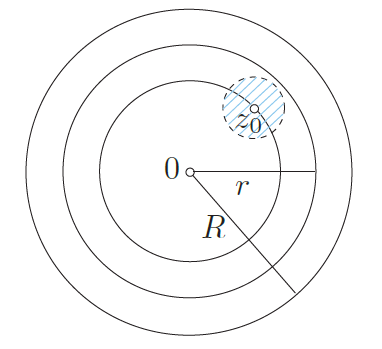
\includegraphics[width=0.3\textwidth]{./SaltChapter/fig-4-0-3}
\end{center}
%\caption{$\mathbb C$에 정의된 제곱급수의 수렴영역}
%\label{fig-4-0-3}
\end{figure*}

$\epsilon>0$이라 하자.
$\Sum_{n=1}^\infty nc_nr^{n-1}$이 절대수렴하므로
다음을 만족하는 $N$이 존재한다.
\[
\Sum_{n=N}^\infty \left| nc_nr^{n-1}\right| < \dfrac \epsilon4.
\]
이제부터 $N$을 고정하자.
$f(z) - f(z_0) = \Sum_{n=1}^\infty c_n(z^n - z_0^n)$이므로,
$z\ne z_0$에 대하여
\[
\dfrac{f(z)-f(z_0)}{z-z_0}  
= \sum_{n=1}^\infty c_n \dfrac{z^n-z_0^n}{z-z_0}
= \sum_{n=1}^\infty c_n \left(
z^{n-1} + z^{n-2}z_0 + \cdots + z_0^{n-1} \right).
\]
따라서,
\[
\dfrac{f(z)-f(z_0)}{z-z_0}   - g(z_0)
= \sum_{n=1}^\infty c_n \dfrac{z^n-z_0^n}{z-z_0}
= \sum_{n=1}^\infty c_n \left(
z^{n-1} + z^{n-2}z_0 + \cdots + z_0^{n-1} - nz_0^{n-1}\right).
\]
이 급수에서 처음 $N-1$개 항의 합을 $S_1$이라 하고
(즉, $n=1$에서 $n=N-1$까지),
$S_2$를 나머지 항의 합이라고 하자.
그러면, $|z|, |z_0| < r$로부터
\[
|S_2| \le \sum_{n=N}^\infty |c_n| 
\left( \underbrace{r^{n-1}+r^{n-1} + \cdots + r^{n-1}}_{n\text{개 항}}
+ nr^{n-1}\right)
= \sum_{n=N}^\infty 2n|c_n|r^{n-1} < \dfrac\epsilon2.
\]
한편,
\[
S_1= \sum_{n=1}^N c_n \left(
z^{n-1} + z^{n-2}z_0 + \cdots + zz_0^{n-2} + z_0^{n-1} - nz_0^{n-1}
\right)
\]
는 $z$의 다항식이며 극한은 다음과 같다.
\begin{align*}
\lim_{z\to z_0} S_1
&= \sum_{n=1}^N c_n \left(
z^{n-1} + z^{n-2}z_0 + \cdots + zz_0^{n-2} + z_0^{n-1} - nz_0^{n-1}
\right) \\
&= \sum_{n=1}^N c_n \left(
nz_0^{n-1}  - nz_0^{n-1} \right) = 0.
\end{align*}
따라서
$|z-z_0|<\delta$이면, $|S_1|< \epsilon/2$가 되는 
양수 $\delta$가 존재한다.
이제 $|z|<r$이고 $0<|z-z_0|< \delta$에 대하여
\[
\left| \dfrac{f(z)-f(z_0)}{z-z_0}   - g(z_0) \right|
\le |S_1| + |S_2| <  \dfrac\epsilon2 + \dfrac\epsilon2 = \epsilon.
\]
이로써 $f'(z_0) = g(z_0)$가 증명된다.
\hfill $\square$

\begin{salt_remark} \label{rem-4-1}
$(c_n)_{n\in\mathbb N}$이 실수열일 때,
실제곱급수
\[
\sum_{n=0}^\infty c_nx^n
\]
\end{salt_remark}
를 생각해보자. 실해석의 결과로부터 어떤 $R>0$이 존재하여
이 제곱급수는 구간 $(-R, R)$에서 수렴하고
$\mathbb R \setminus [-R,R]$에서 발산한다.
정리 \ref{thm-4-1}과 \ref{thm-4-3}로부터
실변수 $x$를 복소변수 $z$로 바꾸면 실제곱급수의 결과가 
복소평면의 원판 $|z|<R$에 정의된 복소해석함수로 확장됨을 알 수 있다.
따라서
실해석함수(즉, 국소적으로 제곱급수 전개를 갖는 실변수함수)는
복소해석함수를 실수축에 제한한 것으로 볼 수 있다.
이 결과로 실해석학과 복소해석학의 세계를 연결하는
상호작용을 엿볼 수 있다
(우리는 코시-리만 방정식을 공부하면서 이미 이러한 사례를 살펴 본 바 있다).

앞의 결과를 반복하면 다음을 쉽게 얻는다.

\begin{salt_corollary}\label{coro-4-1}
$R>0$이고, $f(z):= \Sum_{n=0}^\infty c_n z^n$이 $|z|<R$에서 수렴한다고 하자.
그러면, $k\ge1$에 대하여
\begin{equation}\label{eq-4-1}
f^{(k)}(z) = \sum_{n=k}^\infty n(n-1)(n-2)\cdots (n-k+1)c_nz^{n-k}.
\quad (|z|<R)
\end{equation}
특히, $n\ge0$에 대하여, $c_n = \dfrac1{n!} f^{(n)}(0)$.
\end{salt_corollary}

{\bf 증명}

직접 계산하여 바로 얻을 수 있는 결과이며, 두번째 결과를 얻기 위해
식 \eqref{eq-4-1}에 $z=0$을 대입하면
\[
f^{(k)}(0) = k(k-1)\cdots 1c_k + z \sum{n=k+1}^\infty n(n-1) \cdots (n-k+1)c_n z^{n-k-1}\Big|_{z=0}
= k!c_k
\]
이며, $f(0)=c_0$이다.
\hfill $\square$

이는 $0$을 중심으로 전개한 제곱급수에 한정된 결과가 아니다.
복소수 $z_0$를 택하여 제곱급수
\[
\sum_{n=0}^\infty c_n(z-z_0)^n
\]
를 생각하면, 정리 \ref{thm-4-1}과 \ref{thm-4-3}으로부터
다음 결과를 바로 얻는다.


\begin{salt_corollary} \label{thm-4-2}
제곱급수 $\Sum_{n=0}^\infty c_n(z-z_0)^n$에 대하여
다음 두 가지 중 정확히 하나만 성립한다.
\begin{itemize}
\item[(1)] 모든 $z\in\mathbb C$에 대하여 절대수렴하거나
\item[(2)] 음이 아닌 실수 $R$이 유일하게 존재하여 다음을 만족한다.
\begin{itemize}
\item[(a)] $|z-z_0|<R$인 모든 $z\in\mathbb C$에 대하여 
$\Sum_{n=0}^\infty c_n(z-z_0)^n$이 절대수렴하고,
\item[(b)] $|z-z_0|>R$인 모든 $z\in\mathbb C$에 대하여 
$\Sum_{n=0}^\infty c_n(z-z_0)^n$는 발산한다.
\end{itemize}
\end{itemize}
\end{salt_corollary}

\begin{salt_corollary}\label{coro-4-3}
$z_0\in \mathbb C$, $R>0$이고, 
$f(z):= \Sum_{n=0}^\infty c_n (z-z_0)^n$이 $|z-z_0|<R$에서 수렴한다고 하자.
그러면, $k\ge1$에 대하여
\[
f^{(k)}(z) = \sum_{n=k}^\infty n(n-1)(n-2)\cdots (n-k+1)c_n(z-z_0)^{n-k}.
\quad (|z-z_0|<R)
\]
특히, $n\ge0$에 대하여, $c_n = \dfrac1{n!} f^{(n)}(z_0)$.
\end{salt_corollary}

\begin{salt_remark} [계수의 유일성] \label{rem-4-2}
중심이 $z_0$, 반지름 $R>0$인 열린원판에서
두 제곱급수
\[
\Sum_{n=0}^\infty c_n(z-z_0)^n \quad\text{와}\quad
\Sum_{n=0}^\infty \tilde c_n(z-z_0)^n
\]
가 모두 같은 함수 $f$로 수렴한다고 하자.
그러면 위의 따름정리로부터 모든 $n\ge0$에 대하여
\[
c_n = \dfrac{f^{(n)}(z_0)}{n!} = \tilde c_n.
\]
\end{salt_remark}

\begin{salt_exercise} \label{ex-4-10}
$|z|<1$일 때,
$1^2 + 2^2z + 3^2z^2 + 4^2z^3 + \cdots$의 값은?
\end{salt_exercise}

\begin{salt_exercise} \label{ex-4-11}
제곱급수 $\Sum_{n=0}^\infty c_nz^n$에 대하여 다음 문장의 참, 거짓을 판정하라.
\begin{itemize}
\item[(1)] 급수가 수렴하는  복소수 $z$의 집합은 $\{0\}$이거나, 유한한 반지름을 갖는 열린원판,
또는 복소평면 전체가 되며 다른 경우는 생길 수 없다.
\item[(2)] 제곱급수가 $z=1$에서 수렴하면 $|z|<1$에서 수렴한다.
\item[(3)] 제곱급수가 $z=1$에서 수렴하면 원 $|z|=1$의 모든 점에서 수렴한다.
\item[(4)] 제곱급수가 $z=1$에서 수렴하면 $z=-1$에서 수렴한다.
\item[(5)] 제곱급수가 원점이 중심이고 반지름이 유한한 열린원판에서 수렴하면
원판의 경계(즉, 원판을 둘러싸는 원)의 전체 또는 일부에서도 수렴할 수 있으나
그 이외의 점에서는 수렴할 수 없다.
\item[(6)] 수렴하는 범위가 닫힌원판 $|z|\le 1$ 전체인 제곱급수가 존재한다.
\item[(7)] 제곱급수가 $z=i$에서 발산하면, $z=1+i$에서도 발산한다.
\end{itemize}
\end{salt_exercise}

\section{테일러 급수} \label{section-4-3}

앞 절에서 수렴반경이 $R$인 복수제곱급수
\[
\sum_{n=0}^\infty c_n(z-z_0)^n
\]
은 영역 $|z-z_0|<R$에서 복소해석함수가 됨을 살펴보았다.
이 절에서는 역으로 $f$가 원판 $|z-z_0|<R$에서 복소해석함수이면
\[
f(z) = \sum_{n=0}^\infty c_n (z-z_0)^n \quad (|z-z_0|<R)
\]
임을 보일 것이다. 여기서 계수 $c_n$은 $f$로부터 결정된다.
따라서 영역 $D$에 정의된 복소해석함수 $f$는 임의의 점 $z_0\in D$의 근방에서
제곱급수 전개를 갖는다.

\begin{salt_theorem}\label{thm-4-4}
$f$가 $D(z_0,R) := \{ z\in \mathbb C \,:\, |z-z_0| <R \}$에서 복소해석함수이면,
$z\in D(z_0,R)$에 대하여
$f(z) = c_0 + c_1(z-z_0) + c_2(z-z_0)^2 + c_3(z-z_0)^3+ \cdots$이다.
여기서, $n\ge0$에 대하여
\[
c_n = \dfrac1{2\pi i} \int_C \dfrac{f(\zeta)}{(\zeta-z_0)^{n+1}} d\zeta
\]
이고, $C$는 중심이 $z_0$이고 반지름 $r$ ($0<r<R$)인 원을 반시계방향으로 도는 원이다.
\end{salt_theorem}

\begin{figure*}[h!]
\begin{center}
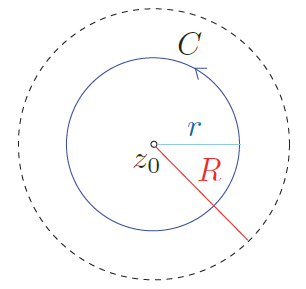
\includegraphics[width=0.3\textwidth]{./SaltChapter/fig-4-0-4}
\end{center}
%\caption{$\mathbb C$에 정의된 제곱급수의 수렴영역}
%\label{fig-4-0-3}
\end{figure*}

{\bf 증명}

$z\in D(z_0, R)$이라 하자.
우선 $|z-z_0|<r<R$인 $r$을 잡고
코시 적분공식을 적용하면
\begin{align*}
f(z) &= \dfrac1{2\pi i}\int_C \dfrac{f(\zeta)}{\zeta-z} d\zeta
= \dfrac1{2\pi i}\int_C \dfrac{f(\zeta)}{\zeta-z_0+z_0-z} d\zeta \\
&= \dfrac1{2\pi i}\int_C \dfrac{f(\zeta)}{(\zeta-z_0)\left(1- \dfrac{z-z_0}{\zeta-z_0}\right)} d\zeta.
\end{align*}
$w:=\dfrac{z-z_0}{\zeta-z_0}$라 하면,
$|w| = \dfrac{|z-z_0|}r <1$이므로
\begin{align*}
\dfrac1{1-\dfrac{z-z_0}{\zeta-z_0}} = \dfrac1{1-w}
& = 1+ w + w^2 + w^3 + \cdots + w^{n-1} + \dfrac{w^n}{1-w} \\
&= 1 + \dfrac{z-z_0}{\zeta-z_0} + \cdots + \dfrac{(z-z_0)^{n-1}}{(\zeta-z_0)^{n-1}}
+ \dfrac{(z-z_0)^n}{(\zeta-z_0)^{n-1}(\zeta-z)}.
\end{align*}
이 결과를 종합하면
\begin{align*}
f(z) &= \dfrac1{2\pi i}\int_C f(\zeta) \left(
\dfrac1{\zeta-z_0} + \cdots + \dfrac{(z-z_0)^{n-1}}{(\zeta-z_0)^{n}}
+ \dfrac{(z-z_0)^n}{(\zeta-z_0)^{n}(\zeta-z)} \right) d\zeta \\
&= c_0 + c_1(z-z_0) + \cdots + c_{n-1}(z-z_0)^{n-1} + R_n(z),
\end{align*}
여기서 
\[
R_n(z) := \dfrac1{2\pi i} \int_C \dfrac{f(\zeta)(z-z_0)^n}{(\zeta-z_0)^n(\zeta-z)}d\zeta.
\]
이제 $n\to\infty$일 때, $R_n(z)$가 $0$으로 수렴하는 것을 보이면 증명이 끝난다.
콤팩트 집합의 연속 실함수이므로 $|f|$는 원 위에서 유계이다.
즉, 원 위의 모든 $\zeta\in C$에 대하여 $|f(\zeta)|<M$을 만족하는 상수 $M>0$이 존재한다
(약간 왜곡하면 경로 $C$를 생각할 때, 점 $C(t)$의 집합 ($t\in [0,2\pi]$)으로 간주할 수 있다).
또한 $\zeta\in C$에 대하여
\[
\left| \dfrac{(z-z_0)^n}{(\zeta-z_0)^n}\right| 
= \left( \dfrac{|z-z_0|}r \right)^n
\stackrel{n\to\infty}{\longrightarrow} 0.
\]
한편 $\zeta\in C$에 대하여 $1/|\zeta-z|$는 어떻게 되는가?
어떤 수로 유계임을 보일 수 있는가?
아래 그림을 보면 실제로 원 $C$와  $z$의 거리의 역수로 유계이다.

\begin{figure*}[h!]
\begin{center}
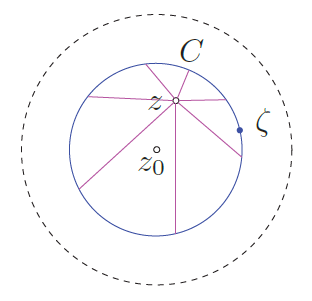
\includegraphics[width=0.3\textwidth]{./SaltChapter/fig-4-0-5}
\end{center}
%\caption{$\mathbb C$에 정의된 제곱급수의 수렴영역}
%\label{fig-4-0-3}
\end{figure*}

$|\zeta-z| = |\zeta-z_0-(z-z_0)| \ge
|\zeta-z_0| - |z-z_0| = r - |z-z_0|$이므로
\[
|R_n(z)| \le \left( \dfrac{|z-z_0|}r \right)^n \dfrac M{r-|z-z_0|} 
\stackrel{n\to\infty}{\longrightarrow} 0.
\]
따라서 제곱급수 $c_0 + c_1(z-z_0) + c_2(z-z_0)^2 + c_3(z-z_0)^3+ \cdots$는
$f(z)$로 수렴한다.
지금까지 결과로
\[
c_n = \dfrac1{2\pi i} \int_C \dfrac{f(\zeta)}{(\zeta-z_0)^{n+1}} d\zeta
\]
이 $|z-z_0|<r<R$인 $r$에서 성립한다는 것만을 보였다.
하지만 코시 적분정리를 사용하면 적분이 $r$에 무관함을 알 수 있고
$r\in (0,R)$이 다음을 만족하도록 선택할 수 있다.
\begin{itemize}
\item[(1)] $\dfrac{f(\cdot)}{(\cdot - z_0)^{n+1}}$이 
$0<|z-z_0|<R$인 뚫린 원판 $D_*(z_0,R)$에서 복소해석함수이다.
\item[(2)] $C$이외의 다른 경로로 중심이 $z_0$, 반지름 $\tilde r\in (0,R)$인 원 $\tilde C$를 잡으면
$C$와 $\tilde C$는 $D_*(z_0,R)$에서 호모토픽하다. 
\end{itemize}
이로써 증명이 완성된다. \hfill $\square$

한편 정리 \ref{thm-4-3}으로부터
\[
f(z) = \sum_{n=0}^\infty c_n(z-z_0)^n
\quad (|z-z_0| <R)
\]
로 정의하면 $n\ge0$에 대하여 $c_n = \dfrac{f^{(n)}(z_0)}{n!}$이다.
이상에서 적분으로 주어진 계수 $c_n$에 대한  다른 표현식을 얻었다.
하지만 임의의 원판에서 제곱급수를 전개할 때 계수는 유일하게 결정된다.
따라서 두 표현식은 같은 결과가 된다는 것을 기억하면 다음 결과를 얻는다.

\begin{salt_corollary}(테일러\footnote{
이 급수 전개에 대하여 연구한 학자 중 실해석 함수 관점에서 연구한
브룩 테일러(Brook Taylor, 1685-1731)의 이름이다.
}
 급수) \label{coro-4-4}
\begin{itemize}
\item[(1)] $D$가 영역이고,
\item[(2)] $f:D\to \mathbb C$가 복소해석함수이고,
\item[(3)] $z_0\in D$ 이면,
\end{itemize}
\[
f(z) = f(z_0) + \dfrac{f'(z_0)}{1!}(z-z_0) + \dfrac{f''(z_0)}{2!}(z-z_0)^ 2 
+ \cdots, \quad |z-z_0|<R.
\]
여기서 $R$은 $z_0$를 중심으로 하는 원판 중 영역 $D$에 속하는 가장 큰 열린집합의
반지름이다. 또한,
\begin{equation} \label{eq-4-2}
f^{(n)}(z_0) = \dfrac{n!}{2\pi i}\int_C \dfrac{f(z)}{(z-z_0)^{n+1}}dz.
\end{equation}
\end{salt_corollary}
단, $C$는 $z_0$를 중심으로 하는 반지름 $r$ ($0<r<R$)인 원을 반시계방향으로 회전하는 경로이다.

식 \eqref{eq-4-2}는 (일반화된) 코시 적분공식이라 불린다. 우리는 앞서 $n=0$인 경우(정리 \ref{thm-3-4})와
$n=1$인 경우(정리 \ref{thm-3-6}의 증명)에 대하여 증명했었다.
여기에 더하여 위 결과로부터 임의의 점 $w\in \Delta:=\{z\in\mathbb C\,:\, |z-z_0| <R \}$에 
대하여 다음 식을 얻는다.
\[
f^{(n)}(w) = \dfrac{n!}{2\pi i}\int_C \dfrac{f(z)}{(z-w)^{n+1}}dz.
\]
이는 코시 적분정리로부터 얻어지는데,
우선 $w$를 중심으로 하는 작은 원 $C_\delta$에 대하여 위 식을 증명한 다음
경로 $C$와 $C_\delta$가 $\Delta\setminus \{w\}$-호모토픽이며,
$f(\cdot)/(\cdot-w)^{n+1}$이 $\Delta\setminus \{w\}$에서 복소해석함수임을 이용하여 보일 수 있다.

{\bf 증명}

정리 \ref{thm-4-4}로부터,
중심이 $z_0$이고 $D(z_0,R):= \{ z\in \mathbb C \,:\, |z-z_0|<R\}$가
$D$에 포함되는 가장 큰 열린원판이 되도록 $R$을 선택한다.
\begin{equation}\label{eq-4-3}
f(z) = c_0 + c_1(z-z_0) + c_2(z-z_0)^2 + c_3(z-z_0)^3 + \cdots, \quad
z\in D(z_0,R).
\end{equation}
또한, $n\ge0$에 대하여
\[
c_n = \dfrac1{2\pi i} \int_C \dfrac{f(z)}{(z-z_0)^{n+1}} dz,
\]
여기서 $C$는 $z_0$를 중심으로 하는 반지름 $r$ ($0<r<R$)인 원을 반시계방향으로 회전하는 경로이다.
한편, 따름정리 \ref{coro-4-3}에 의하여
제곱급수는 무한번 미분가능하고, $n\ge0$에 대하여
\[
\dfrac1{n!}f^{(n)}(z_0) = c_n
\]
이므로 원하는 결과를 얻는다. \hfill $\square$

요약하면, 
$f$가 영역 $|z-z_0|<R$에 정의된 복소해석함수이면, $|z-z_0|<R$에서
\[
f(z) = \sum_{n=0}^\infty \left( \dfrac 1{2\pi i}
\int_C \dfrac{f(\zeta)}{(\zeta - z_0)^{n+1}}d\zeta \right)\cdot
(z-z_0)^n
=  \sum_{n=0}^\infty \dfrac{f^{(n)}(z_0)}{n!} (z-z_0)^n,
\]
여기서 $C(t) = z_0 + r\exp (it)$ ($t\in[0,2\pi]$)이고 $r$은
$0<r<R$을 만족하는 임의의 실수이다.

\begin{salt_example} \label{exxample-4-3}
지수함수 $f$, $z\mapsto f(z):=\exp z$는 전해석함수이다.
따라서 적당한 계수 $c_n$에 대하여
\[
\exp z = \sum_{n=0}^\infty c_nz^n \quad (z\in \mathbb C)
\]
로 쓸 수 있다. 
다음 식으로 주어진 계수들을 실제로 구하면?
\[
c_n = \dfrac1{n!}f^{(n)}(z_0), \quad n\ge 0
\]
$\dfrac d{dz}\exp z = \exp z$이고$f^{(n)}(0)=1$이므로
\[
f(z) = \sum_{n=0}^\infty \dfrac{f^{(n)}(0)}{n!} (z-0)^n 
=\sum_{n=0}^\infty \dfrac{1}{n!} z^n\quad (z\in\mathbb C).
\]
\hfill $\diamondsuit$
\end{salt_example}

\begin{salt_example} \label{exxample-4-4}
$f(z) = \Log(z)$로 정의된 함수 $f$는 $\mathbb C\setminus (-\infty,0]$에서 
복소해석함수이다. 이 잘린 평면에서 $z_0=1$을 중심으로 가장 큰 열린원판을 잡으면
$D = \{z\in\mathbb C\,:\, |z-1|<1\}$이다.
\[
f^{(n)}(z_0) = \dfrac{(-1)^n(n-1)!}{z_0^n} = (-1)^n (n-1)!
\]
이므로 $|w|<1$에 대하여
\[
\Log (1+w) = w - \dfrac {w^2}{2} + \cdots + \dfrac{(-1)^nw^n}n + \cdots
\]
를 얻는다. \hfill $\diamondsuit$
\end{salt_example}

\begin{salt_exercise} \label{ex-4-12}
$z\in\mathbb C$에 대하여 다음 등식을 보여라.
\[
\sin z = z - \dfrac{z^3}{3!} + \dfrac{z^5}{5!} - \cdots,
\quad
\cos z = 1 - \dfrac{z^2}{2!} + \dfrac{z^4}{4!} - \cdots.
\]
\end{salt_exercise}

\begin{salt_exercise} \label{ex-4-13}
$z_0=1$을 중심으로 하여
다항식 $z^-z^4 + z^2 -1$의 테일러 급수를 구하라.
\end{salt_exercise}

\begin{salt_exercise} \label{ex-4-14}
함수 $f$가 다음과 같을 때 테일러 급수 $\Sum_{n=0}^\infty c_nz^n$의 계수 $c_n$을 구하라.
\begin{itemize}
\item[(1)] $f(z) = \dint_{\gamma_{0z}} \exp(\zeta^2)d\zeta$ ($z\in\mathbb C$),
단, $\gamma_{0z}$는 $0$에서 $z$까지 연결하는 직선 경로이다. \\
힌트: $f'(z) = \exp(z^2)$.
\item[(2)] $f(z) = \dfrac{z^2}{(z+1)^2}$ ($z\in \mathbb C\setminus \{-1\}$). \\
힌트: $|z|<1$에 대하여, $\dfrac1{z+1} = 1- z + z^2 - \cdots$.
\end{itemize}
\end{salt_exercise}

일반화된 코시 적분정리에서 얻어지는 결과를 더 살펴보자.

\begin{salt_corollary}[코시 부등식] \label{coro-4-5}
\ 
\begin{itemize}
\item[(1)] $f$가 $D(z_0, R):= \{z \in \mathbb C\,:\, |z-z_0| <R \}$에 정의된
복소해석함수이고,
\item[(2)] 모든 $z\in D(z_0,R)$에 대하여 $|f(z)|\le M$이면,
\end{itemize}
$n\ge0$에 대하여  \ $|f^{(n)}(z_0)| \le \dfrac{n! M}{R^n}$.
\end{salt_corollary}

{\bf 증명}

$C$가 $z_0$를 중심으로 하고 반지름이 $r<R$인 원이라 하자. 그러면
\begin{align*}
|f^{(n)}(z_0)| &= \left| \dfrac{n!}{2\pi i} \int_C \dfrac{f(z)}{(z-z_0)^{n+1}}dz \right| \\
&\le \dfrac{n!}{2\pi} \max_{z\in C} \left| \dfrac{f(z)}{(z-z_0)^{n+1}} \right| \cdot 
2\pi r = \dfrac{n!}{2\pi} \dfrac{M}{r^{n+1}}2\pi r = \dfrac{n! M}{r^n}.
\end{align*}
극한 $r\nearrow R$을 취하면 원하는 결과를 얻는다. 
\hfill $\square$

\begin{salt_exercise} \label{ex-4-15}
$f$가 전해석함수이고 모든 $z\in\mathbb C$에 대하여
$|f(z)| \le < M|z|^n$을 만족하는  $M>0$과 정수 $n\ge0$가 존재한다고 가정하자.
코시 부등식을 이용하여 모든 $z$에 대하여 $f^{(n+1)}(z) = 0$을 증명하고
$f$는 $n$차 이하 다항식임을 보여라. $n=0$일 때는 어떤 결론을 얻는가?
\end{salt_exercise}

\begin{salt_exercise} \label{ex-4-16}
$C$가 원점을 중심으로 반지름 $1$인 원을 반시계방향으로 도는 원형 경로일 때,
$\dint_C \dfrac{\sin z}{z^{2013}}dz$를 구하라.
\end{salt_exercise}

\section{근의 분류}

영역 $D$에서  $f: D\to \mathbb C$가 복소해석함수라고 하자.
항등적으로 $0$이 아닌 함수 $f$의 근은 어떤 모습일까?
($f(z_0)=0$를 만족하는 점 $z_0\in D$를 $f$의 {\bf 근(zero)}이라 한다)
이 절에서는 이 문제의 답으로 근들이 ``고립''되어 있음을 보일 것이다.
연속함수의 경우는 이러한 일이 일어나지 않는다. 
연속함수는 복소해석함수만큼 엄격한 조건을 갖지 않기 때문에
의 근이 고립될 필요가 없다.

\begin{salt_example}\label{example-4-5}
\
\begin{itemize}
\item[(1)] $\exp z$는 $\mathbb C$에서 근을 갖지 않는다.
실제로, 모든 $z\in \mathbb C$에 대하여 $|\exp(z)| = e^{\Re(z)} >0$이다.
\item[(2)] $\cos z - 3$은 $\mathbb C$에서 무한이 많은 근 
$2\pi n \pm i \log(3+2\sqrt{2})$ ($n\in\mathbb Z$)
을 갖는다.
모든 근은 수평선에 분포하고 인접한 근과의 간격은 $2\pi$이다.
계산방법은 연습문제 \ref{ex-1-38}을 참고하라.
\item[(3)] 다항식 $p(z) = (z+1)^3z^9(z-1)^9$은 $-1, 0, 1$에서 근을 갖는다. 
\hfill $\diamondsuit$
\end{itemize}
\end{salt_example}

$p$가 항등적으로 $0$이 아닌 다항식이고 $p(z_0)=0$이면
나눗셈정리에 따라 
\[
p(z) = (z-z_0) q(z)
\]
을 만족하는 다항식 $q$(몫)가 존재한다
(즉, 나머지가 $0$이다). 
이제 다음 두 가지  가능성을 생각할 수 있다.
\begin{itemize}
\item[$1^\circ$] $q(z_0) \ne0$. 그러면 $z_0$는 $p$의 고립 근이다.
\item[$2^\circ$] $q(z_0) =0$. 그러면 $p$를 $q$로 바꾸어 위 과정을 반복한다.
\end{itemize}

궁극적으로 적당한 $m\ge1$에 대하여 $p(z) = (z-z_0)^mq(z)$이고  $q(z_0)\ne0$에 도달한다.
이 때 $m$을 ($p$의 근) $z_0$의 중복도(multiplicity) 또는 차수(order)라 부른다.
아래 명제 \ref{prop-4-1}에서 복소해석함수 $f$에서도 (다항식 $p$를 대체하여)
같은 종류의 결과를 얻을 수 있음을 보일 것이다.
다만, 결과가 다항식 $q$ 대신 복소해석함수 $g$로 마무리된다는 것만 다르다.
이는 아주 놀라운 결과는 아니다. 왜냐하면, 제곱급수는 다항식으로부터 유추될 수 있고
임의의 복소해석함수는 국소적으로 제곱급수 전개가 가능하기 때문이다.
우선 다음 정의를 만들자.

\begin{salt_definition} \label{def-4-2}
$D$가 영역이고, $f:D\to\mathbb C$가 $D$에서 복소해석함수라고 하자.
$f(z_0)=0$이면 점 $z_0\in D$를 $f$의 {\bf 근}이라고 한다.
다음 조건을 만족하는 가장 작은 자연수를 $m\in\mathbb N$이 존재하면,
\begin{itemize}
\item[(1)] $f^{(m)}(z_0) \ne 0$이고,
\item[(2)] $f(z_0) = \cdots = f^{(m-1)}(z_0) = 0$.
\end{itemize}
$z_0$는 $f$의 {\bf $m$ 중근}이라 한다
(관습적으로 $f^{(0)} := f$라 한다).
\end{salt_definition}

그러면, 복소해석함수의 근의 분류에 대한 다음 결과를 얻는다.

\begin{salt_prop} [근의 분류] \label{prop-4-1}
\
\begin{itemize}
\item[(1)] $D$가 영역이고,
\item[(2)] $f:D\to\mathbb C$가 $D$에서 복소해석함수이고,
\item[(3)] $z_0 \in D$가 $f$의 근이라고 하자.
\end{itemize}
그러면, 정확히 다음 두 가지 가능성이 있다.
\begin{itemize}
\item[$1^\circ$] 양수 $R$이 존재하여 $|z-z_0|<R$인 모든 $z$에 대하여
$f(z)=0$.
\item[$2^\circ$] $m\in\mathbb N$이 존재하여
 $z_0$가 $f$의 $m$중근이다. 또한, 
 $g(z_0)\ne0$이고 모든 $z\in D$에 대하여 $f(z) = (z-z_0)^mg(z)$인
 복소해석함수 $g:D\to\mathbb C$가 존재한다.
\end{itemize}
\end{salt_prop}

$2^\circ$의 경우 $g$가 연속이고 $g(z_0)\ne0$이므로
$g$는 $z_0$를 중심으로 하는 작은 원판 $\Delta$에서 $0$이 아니며,
$z\in \Delta\setminus \{z_0\}$에서 $f(z) = (z-z_0)^mg(z) \ne 0$이므로
$f$는 $\Delta\setminus \{z_0\}$에서 $0$이 아니다.
따라서 $z_0$는 $\Delta$에서 $f$ 의 유일한 근이다. 즉, 고립된 근이다.

한편, 앞으로 보게 될 항등정리에 따르면
$1^\circ$의 경우는 영역 $D$ 전체에서 $f\equiv 0$이다.

{\bf 증명}

중심이 $z_0$이고 반지름 $R>0$인 원판에서 $f$의 제곱급수 전개를 하면,
\[
f(z) = c_0 + c_1(z-z_0) + c_2(z-z_0)^2 + c_3(z-z_0)^3 + \cdots, \quad
(|z-z_0| <R).
\]
$f(z_0)=0$이므로, $c_0=0$임을 바로 알 수 있다. 
이제 정확히 두 가지 가능성이 있다.
\begin{itemize}
\item[$1^\circ$] 모든 $c_n$이 $0$이다. 그러면, $|z-z_0| <R$에서 $f(z)=0$이다.
\item[$2^\circ$] $c_m\ne 0$인 가장 작은 $m\ge1$이 존재한다.
그러면 $c_0=c_1=\cdots = c_{m-1}=0$이고,
\[
c_n = \dfrac{f^{(n)}(z_0)}{n!}, \quad n\ge0
\]
로부터 $z_0$는 $m$ 중근이다.
또한, 제곱급수 전개로부터 $|z-z_0|<R$에 대하여
\begin{equation} \label{eq-4-4}
f(z) = c_m(z-z_0)^m + c_{m+1}(z-z_0)^{m+1} + \cdots
= (z-z_0)^m \sum_{k=0}^\infty c_{m+k} (z-z_0)^k.
\end{equation}
따라서 $g:D\to \mathbb C$를 
\[
g(z) = \begin{cases}
\dfrac{f(z)}{(z-z_0)^m}, & z\ne z_0, \\
\Sum_{k=0}^\infty c_{m+k} (z-z_0)^k, & |z-z_0|<R
\end{cases}	
\]
로 정의하면,
식 \eqref{eq-4-4}로부터 두 가지 조건을 모두 만족하는 경우
두 가지 경우의 계산결과가 일치하므로
$g$는 잘 정의된다. 추가적으로 다음 결론을 얻는다.
\begin{itemize}
\item[(1)]  $g$는 $D$에서 복소해석함수이다. $z\ne z_0$에서
$f$와 $1/(\cdot - z_0)^m$이 $D\setminus \{z_0\}$에서 복소해석함수이므로
$|z-z_0|<R$에 대하여 제곱급수로 정의된 $g$는 복소해석함수이다.
\item[(2)] $g(z_0) = c_m\ne 0$ ($m$의 정의에서)
\item[(3)] 식 \eqref{eq-4-4}로부터 $z\in D\setminus \{z_0\}$에 대하여
$f(z) = (z-z_0)^mg(z)$. 한편, $z=z_0$이면 양변이 $0$이 된다.
따라서 모든 $z\in D$에 대하여 $f(z) = (z-z_0)^mg(z)$이 성립한다.
\item[(4)] $z_0$는 $m$ 중근이다.
왜냐하면, 모든 $n$에 대하여 $c_n = f^{(n)}(z_0)/n!$이므로
$c_m \ne 0$이고, $c_0 = c_1 = \cdots = c_{m-1}= 0$.
\end{itemize}
\end{itemize}
이상에서 정리가 증명된다. \hfill $\square$

\begin{salt_example} \label{example-4-6}
\
\begin{itemize}
\item[(1)] $n\in \mathbb Z$에 대하여 $n\pi$는 $\sin z$의 근이다.
$\sin z$를 실수축에 한정하면 $n\pi$의 근방에서 
$\sin z$가 항등적으로 $0$이 아님을 알 수 있다.
$\sin z$의 근으로서 $n\pi$는 몇 중근인가?
$\sin `z = \cos z$이고, $\cos z \Big|_{z=n\pi}= (-1)^n \ne 0$이므로
$n\pi$는 $\sin z$의 근이지만 중근이 아니다.
\item[(2)] $\exp(0^2) -1 = 1-1 = 0$이므로
$\exp (z^2) -1$은 근으로 $0$을 갖는다.
몇 중근일까?
\[
\exp (z^2) = 1 + \dfrac{z^2}{1!} + \dfrac{z^4}{3!} + \cdots,
\quad z\in \mathbb C
\]
이고, $\exp(z^2) -1 = z^2g(z)$ ($z\in \mathbb C$),
여기서 $g(z):= \dfrac1{1!} + \dfrac{z^2}{2!} = \cdots$.
$g$는 $\mathbb C$에서 수렴하는  제곱급수로 전개되므로
전해석함수이다. 또한, $g(0)=1\ne 0$이다.
따라서 $0$은 $\exp(z^2) -1$의 2중근이다.
다른 방법으로 보일 수도 있다.
\begin{align*}
\dfrac{d}{dz} (\exp(z^2)-1) \Big|_{z=0} 
&= (\exp(z^2))\cdot 2z  \Big|_{z=0}  = 0, \\
\dfrac{d^2}{dz^2} (\exp(z^2)-1)\Big|_{z=0} 
&=  (\exp(z^2))\cdot 2 \Big|_{z=0}  +  (\exp(z^2))\cdot (2z^2)  \Big|_{z=0}  \\
&= 2\ne 0.
\end{align*}
$\exp(z^2) -1$의 근으로서 $0$은 이중근이다.
\end{itemize}
\end{salt_example}

\begin{salt_exercise} \label{ex-4-17}
$D$가 영역이고, $m\in \mathbb N$, $R>0$, $z_0\in D$라고 하자.
복소해석함수 $f,g: D\to \mathbb C$가 $g(z_0)\ne0$이고
$|z-z_0|<R$에 대하여 $f(z) = (z-z_0)^m g(z)$이면,
$z_0$가 $f$의 $m$ 중근임을 증명하라.
\end{salt_exercise}

\begin{salt_exercise} \label{ex-4-18}
함수 $f$를 다음과 같이 정의할 때 $f$의 근 $z_0$의 차수는?
\begin{itemize}
\item[(1)]  $z_0 = i$, $f(z) = (1+z^2)^4$.
\item[(2)]  $z_0 = 2n\pi i$ ($n$은 정수), $f(z) = \exp z -1$.
\item[(3)] $z_0=0$, $f(z) = \cos z - 1 + \dfrac12(\sin z)^2$.
\end{itemize}
\end{salt_exercise}

\begin{salt_exercise} \label{ex-4-19}
$f$가 원 $\gamma$를 내부에 포함하는 원판에서 복소해석함수라고 하자.
$f$의 근 $z_0$의 차수는 1이고,
$z_0$는 원 $\gamma$의 내부에 있다.
다음을 증명하라.
\[
z_0 = \dfrac1{2\pi i} \int_\gamma \dfrac{zf'(z)}{f(z)} dz.
\]
\end{salt_exercise}

\begin{salt_exercise} \label{ex-4-20}
$f$가 영역 $D$에서 복소해석함수이고 $z_0\in D$에서
차수 $m$의 근을 갖는다고 하자.
함수 $z \mapsto (f(z))^2$은 차수 $2m$의 근을 가지며,
$f'$은 차수 $m-1$의 근을 가짐을 보여라.
\end{salt_exercise}

\begin{salt_exercise} \label{ex-4-21}
복소 연속함수의 경우는 명제 \ref{prop-4-1}의 복소해석함수에 대한
이분법적 결론을 적용할 수 없다. 
$f:\mathbb C \to \mathbb C$에 대하여 
$0$이  고립된 근도 아니며 $f$가 $0$을 포함하는 작은 원판에서  
항등적으로 $0$이 되지 않는 예를 보여라.
\end{salt_exercise}

\section{항등정리}

이 절에서는 복소해석함수의 엄밀성을 다시 강조하는 항등정리 학습한다.
개략적으로 말하자면
항등적으로 $0$이 아닌 복소해석함수는 정의역에서 근의 집적점(accumulation)을 갖지 않는다.

\begin{salt_theorem} \label{thm-4-5}
\
\begin{itemize}
\item[(1)] $D$가 영역이고,
\item[(2)] $f:D\to\mathbb C$가 $D$에서 복소해석함수이고,
\item[(3)] $f$의 서로 다른 근으로 이루어진 수열 $(z_n)_{n\in\mathbb N}$이 $z_*\in D$로 수렴한다면,
\end{itemize}
$f$는 $D$에서 항등적으로 $0$이다.
\end{salt_theorem}

{\bf 증명}

우선 $z_*$도 $f$의 근이 됨을 보이자.
$f$의 연속성으로부터
\[
f(z_*) = f\left(\lim_{n\to\infty} z_n \right) = \lim_{n\to\infty}f( z_n) 
= \lim_{n\to\infty} 0 = 0.
\]

$z_*$를 중심으로 반지름 $r>0$인 어떤 원판 $\Delta$에서 $f\equiv0$임을 보아자.
그렇지 않다면, $z_*$가 차수 $m$의 근이라고 하자.
$z\in \Delta$에 대하여
$f(z)=(z-z_*)^mg(z)$이고 $g(z)\ne0$이다.
하지만 $n$을 크게 잡을 수 으면 $\Delta$에 속하게 되고
$0 = f(z_n) = (z_n-z_0)^m g(z_n) \ne 0$가 되어 모순이다.

다음으로 $D$에서 $f\equiv 0$임을 보이자.
어떤 점 $w\in D$에서 $f(w)\ne0$라고 가정하자.
그러면 $z_*$와 $w$를 잇는 경로 $\gamma :[0,1] \to D$를 만들 수 있다
($\gamma(0)=z_*$, $\gamma(1)=w$).
집합 $S:=\{t\in[0,1]\,:\, f(\gamma(\tau))=0, 0\le \tau \le t \}$의
상한을 $T:=\sup S$라 하자. $S$가 공집합이 아니기 때문에 (적어도 $0$은 $S$에 속한다)
$\sup S$가 존재함을 알 수 있고
$S$는 위로 유계이다 ($1$을 넘지 못한다). 
그렇다면 $T$의 값은? 변수 $t$를 시간이라고 생각하여
시간 $t=0$에 $z_*$에서 출발하여 경로 $\gamma$를 따라 움직여
시간 $t=1$에 $w$에 도착한다고 하면,
$T$는 경로를 따라 움직일 때 함수 $f$의 값이 $0$을 유지하는 가장 큰 시간을 의미한다.
$T=1$이라면 증명이 끝난다. 왜냐하면 $f$의 연속성에서 $f(w)=f(\gamma(T))=0$이기 때문이다.
따라서 $T<1$이라 하자.
그러면 연속성에서 $f(\gamma(T))=0$이다. 
\begin{figure*}[h!]
\begin{center}
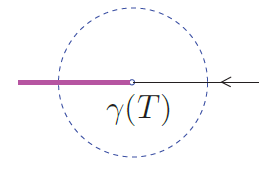
\includegraphics[width=0.3\textwidth]{./SaltChapter/fig-4-0-6}
\end{center}
%\caption{$\mathbb C$에 정의된 제곱급수의 수렴영역}
%\label{fig-4-0-3}
\end{figure*}

그런데 $\gamma(T)$는 $f$의 고립된 근이 아니므로
$\gamma(T)$를 중심으로 적당한 반지름 $\delta$의 원판에서
 $f(z)=0$이다. 즉, 
 $t$ 를 $T$에 가깝게 잡아 $|\gamma(t) - \gamma(T)|<r$을 만족하면
 $T$보다 큰 $t$에 대하여 $f(\gamma(t))=0$이 된다.
이는 $T$의 정의에 모순이다. 따라서 $T$는 $1$보다 작을 수 없어 증명이 끝난다.
\hfill $\square$

\begin{salt_example} \label{example-4-7}
$\cos z$와 $\sin z$의 정의로부터 모든 복소수 $z\in \mathbb C$에 대하여
$(\cos z)^2 + (\sin z)^2 = 1$임을 이미 알고 있다.
여기서는 정리의 결과를 이용하여 이를 증명해보자.
$f:\mathbb C \to \mathbb C$를 $f(z) = (\cos z)^2 + (\sin z)^2 - 1$로
정의하자. 그러면 $f$는 전해석함수이다. 또한
모든 $x\in \mathbb R$에 대하여 $ f(x) = (\cos x)^2 + (\sin x)^2 - 1 = 0$이다.
이제 정리를 적용하면 $\mathbb C$에서 $f\equiv 0$임을 알 수 있다.
\end{salt_example}

정리로부터 다음 결과를 바로 얻는다.

\begin{salt_corollary} [항등정리] \label{coro-4-6}
\
\begin{itemize}
\item[(1)] $D$가 영역이고,
\item[(2)] $f,g:D\to\mathbb C$가 $D$에서 복소해석함수이고,
\item[(3)] $D$의 서로 다른 점으로 만든 수열 $(z_n)_{n\in\mathbb N}$이 $z_*\in D$로 수렴하고,
$f(z_n) = g(z_n)$이면,
\end{itemize}
모든 $z\in D$에 대하여 $f(z) = g(z)$이다.
\end{salt_corollary}

{\bf 증명}

$z\in D$에 대하여
$h:D\to\mathbb C$를 $h(z) = f(z) - g(z)$로 정의하고
$z_n$을 복소해석함수 $h$의 근이라 하자.
정리의 결과로부터 $h$는 $D$에서 항등적으로 $0$이 되므로 증명이 끝난다.\hfill $\square$

\begin{salt_example} \label{example-4-8}
함수 $\exp:\mathbb C \to \mathbb C$
\[
\exp z = \exp(x+iy) := e^x (\cos y + i\sin y), \quad
z + x+iy\in \mathbb C
\]
는  전해석함수이고, $x\in \mathbb R$에서 $\exp x = e^x$를 만족한다.
다시 말하면, $\exp$ 함수는 실수에 정의된 지수함수를 복소수 전해석함수로 확장한 것이다.
전해석함수로 확장하는 다른 방법이 있을까? 그렇지 않다는 것을 보이자.
$g:\mathbb C \to \mathbb C$를  $x\in \mathbb R$에서 $g(x)=e^x$를 만족하는
전해석함수라고 가정하자.
그러면,
\[
\text{모든 } x\in \mathbb R \text{에 대하여 } \exp x = g(x).
\]
특히, 
\[
\exp\left(\dfrac1n\right)=  g\left(\dfrac1n\right), \quad n\in\mathbb N
\]
이고 $1/n \to 0\in \mathbb C$이다.
따라서 항등정리에 의해  모든 $z\in \mathbb C$에 대하여 $\exp z = g(z)$이다.
따라서 실수로 한정했을 때 $e^x$가 되는 전해석함수는 유일하다.
이 결과는 \ref{sec-1-4-1}의 복소 지수함수가 자연스러운 정의임을 설명해준다. 
\hfill $\diamondsuit$
\end{salt_example}

\begin{salt_exercise} \label{ex-4-22}
항등정리를 이용하여 모든 $z_1, z_2 \in \mathbb C$에 대하여
\[
\cos(z_1 + z_2) = (\cos z_1)(\cos z_2) - (\sin z_1)(\sin z_2)
\]
이 성립함을 보여라.
$z_1$, $z_2$가 실수인 경우에 성립함을 활용하라.
\end{salt_exercise}

\begin{salt_exercise} \label{ex-4-23}
영역  $D$에 정의된 복소해석함수의 집합을 $\Hol(D)$라 하자.
그러면 $z\in D$와 $f,g\in \Hol(D)$에 대한 점별 연산
\begin{align*}
(f+g)(z) &=f(z)+g(z), \\
(f\cdot g)(z) &=f(z)g(z)
\end{align*}
에 대하여 $\Hol(D)$가 가환환(commutative ring)이 됨을 쉽게 확인할 수 있다.
(가환환 $R$은 두 연산 $+$와 $\cdot$를 가지며
$(R,+)$는 가환군이고 $\cdot$는 교환법칙, 결합법칙을 만족하며
분배법칙도 성립한다. 즉, $a,b,c\in R$에 대하여 $(a+b)\cdot c = a\cdot c + b\cdot c$이다.)
$\Hol(D)$가 정역(integral domain)이 됨을 보여라.
즉, 영인자(zero divisor)를 갖지 않는다. 다시 말해 $f,g\in \Hol(D)$가 $f\cdot g=0$를
만족하면 $f=0$이거나 $g=0$이다.

$\Hol(D)$ 대신 $D$에 정의된 복소 연속함수의 집합 $C(D)$를 생각하면
$C(D)$도 점별 연산에 대하여 가환환이 된다.
$C(D)$도 정역인가?
(이 결과는 연속함수는 복소해석함수만큼 ``엄밀''하지 않음을 보여준다.)
\end{salt_exercise}

\begin{salt_exercise} \label{ex-4-24}
영역 $D$에서 $f,g$가 복소해석함수라 하자.
다음 중 어떤 조건이 영역 전체에서 $f=g$임을 보장하는가?
\begin{itemize}
\item[(1)] 
$D$의 서로 다른 점으로 된 수열 $(z_n)_{n\in\mathbb N}$이 존재하여
모든 $n\in \mathbb N$에서 $f(z_n) = g(z_n)$을 만족한다.
\item[(2)] $D$의 서로 다른 점으로 된 수열 $(z_n)_{n\in\mathbb N}$이 $D$의 한점으로 수렴하고
모든 $n\in \mathbb N$에서 $f(z_n) = g(z_n)$을 만족한다.
\item[(3)] $D$의 서로 다른 두 점 $a,b$를 연결하는 매끄러운 경로 $\gamma$에서
$f=g$이다.
\item[(4)]  $w\in D$이고, 모든 $n\ge0$에 대하여 $f^{(n)}(w) = g^{(n)}(w)$이다.
\end{itemize}
\end{salt_exercise}

\begin{salt_exercise} \label{ex-4-25}
$f$가 전해석함수라고 가정하자.
임의의 점 $z_0\in \mathbb C$에 대한 제곱급수 전개
$f(z) = \Sum_{n=0}^\infty c_n(z-z_0)^n$마다 적어도 하나의 계수가 $0$이다.
$f$는 다항식임을 증명하라.
\end{salt_exercise}

\section{최대절대값정리}

이 절에서는 복소해석학의 중요한 결과인  최대절대값정리를 증명할 것이다.
이는 상수함수가 아닌 복소해석함수 $f:D\to\mathbb C$의 절대값 $|f|$는 영역 $D$에서
최대값을 가질 수 없음을 의미한다.

\begin{salt_theorem} [최대절대값정리] \label{thm-4-6}
\
\begin{itemize}
\item[(1)] $D$가 영역이고,
\item[(2)] $f:D\to\mathbb C$가 $D$에서 복소해석함수이고,
\item[(3)] 모든 $z\in D$에 대하여 $|f(z_0)| \ge |f(z)|$를 만족하는 $z_0\in D$가 존재하면,
\end{itemize}
$f$는 $D$에서 상수함수이다.
\end{salt_theorem}

{\bf 증명}

중심이 $z_0$이고 반지름 $2r$인 원판이 영역 $D$에 포함되는 $r>0$을 잡고,
$C_r$을 $C_r(t) = z_0 + r\exp(it)$ ($t\in [0,2\pi]$)로 정의된 원형 경로라 하자.
그러면, 코시 적분공식에 의해,
\begin{align*}
f(z_0) &= \dfrac1{2\pi i} \int_\gamma \dfrac{f(z)}{z-z_0}dz
=  \dfrac1{2\pi i} \int_0^{2\pi} \dfrac{f(z_0 + r\exp(it))}{r\exp(it)} ir\exp(it)dt \\
&=  \dfrac1{2\pi} \int_0^{2\pi} f(z_0 + r\exp(it))dt
\end{align*}
이며, 여기서 마지막 식은 $C_r$에서 $f$의 ``평균''으로 해석할 수 있다.
모든 $t$에 대하여 $|f(z_0 + r\exp(it))| \le |f(z_0)|$이므로
\begin{align*}
|f(z_0)| = \left|\dfrac1{2\pi} \int_0^{2\pi} f(z_0 + r\exp(it))dt \right| 
&\le \dfrac1{2\pi} \int_0^{2\pi}  \left| f(z_0 + r\exp(it)) \right|  dt \\
& \le \dfrac1{2\pi} \int_0^{2\pi}  \left| f(z_0) \right|  dt  = |f(z_0)|.
\end{align*}
이 식에서 부등호 $\le$는 모두 등호로 바뀔 수 있거 정리하면
\[
 \dfrac1{2\pi} \int_0^{2\pi}  \big( 
 \underbrace{|f(z_0)|  - |f(z_0 + r\exp(it))|}_{\ge0} \big)  dt  = 0.
\]
를 얻는다.
피적분함수가 $0$보다 크거나 같기 때문에 
모든 $t$에 대하여 $|f(z_0 + r\exp(it))|=|f(z_0)|$이다.
$r$을 더 작은 값으로 바꾸어도 같은 결과를 얻는다.
따라서 $f$는 
원판 $\Delta:= \{z \in \mathbb C \,:\, |z-z_0| \le r \}$을
원 $\{ w\in \mathbb C\,:\, |w| = |f(z_0)| \}$위로 보낸다.
연습문제 \ref{ex-2-11}의 결과로부터
$f$는 $\Delta$에서 상수함수이다.
따라서 항등정리를 적용하면 $f$는 $D$ 전체에서  상수함수이다.
\hfill $\square$

\begin{salt_example} \label{example-4-9}
$\mathbb H := \{z\in\mathbb C\,:\, \Re(z)\ge 0\}$를 우측 반평면이라 하고
$f:\mathbb H\to \mathbb C$를 다음과 같이 정의하자.
\[
f(z) =  \dfrac{\exp(-z)}{z+1}, \quad z\in\mathbb H.
\]
그러면 다음 최대값이 존재한다.
\[
\|f\|_\infty := \max_{z\in\mathbb H} |f(z)|.
\]
최대값의 존재성에 대한 우려를 잊고,
일단 존재한다는 가정하에, 최대절대값정리가 어떻게 그 값을 계산하는데 도움을 주는지  살펴보자.
$z_0\in \mathbb H$에서 최대값을 갖는다고 가정하자.
그러면 최대절대값정리로부터 $z_0$의 실수부는 양수가 될 수 없다.
따라서 $z_0 \in i\mathbb R$이고, 어떤 $y_0\in\mathbb R$에 대하여 $z_0=iy_0$라 하자.
한편,
\[
|f(iy)| = \left| \dfrac{\exp(-iy)}{iy+1} \right| = \dfrac1{\sqrt{y^2+1}}, y\in\mathbb R.
\]
따라서
$\|f\|_\infty = \max\limits_{z\in\mathbb H} |f(z)|
= \max\limits_{y\in\mathbb R} |f(iy)| 
= \max\limits_{y\in\mathbb R} \dfrac1{\sqrt{y^2+1}} 
= \dfrac1{\sqrt{0^2+1}} = 1$. \hfill $\diamondsuit$
\end{salt_example}

\begin{salt_exercise} \label{ex-4-26}
영역 $D$에서 $f:D\to \mathbb C$가 상수함수가 아닌 복소해석함수라 하자.
그러면 $z\mapsto |f(z)|$를 최대로 하는 점이 $D$에 존재하지 않음을 보여라.
\end{salt_exercise}

\begin{salt_exercise} [최소절대값정리] \label{ex-4-27}
영역 $D$에서 $f:D\to \mathbb C$가 복소해석함수라 하자.
모든 $z\in D$에 대하여 $|f(z_0)| \le |f(z)|$를 만족하는 $z_0\in D$가 존재한다고 하자.
그러면 $f(z_0)=0$이거나 $f$는 $D$에서 상수함수임을 증명하라.
\end{salt_exercise}

\begin{salt_exercise} \label{ex-4-28}
함수 $f(z)=z^2-2$에 대하여
$\{z\in\mathbb C \,:\, |z|\le 1\}$에서 $|f(z)|$의 최댓값과 최솟값을 구하라.
\end{salt_exercise}

\section{로랑 급수}

로랑(Laurent) 급수는 테일러 급수의 일반화이다. 
테일러 급수
\[
\sum_{n=0}^\infty c_n(z-z_0)^n
\]
는 $z-z_0$의 음의 지수를 갖지 않으며 적당한 원판에서 수렴하는데,
로랑 급수는
\[
\sum_{n\in \mathbb Z} c_n(z-z_0)^n
= \cdots + c_{-1}(z-z_0)^{-1} + c+0 + c_1(z-z_0)^1 + \cdots
\]
는 $z-z_0$의 음의 지수도 갖는다.

\begin{figure*}[h!]
\begin{center}
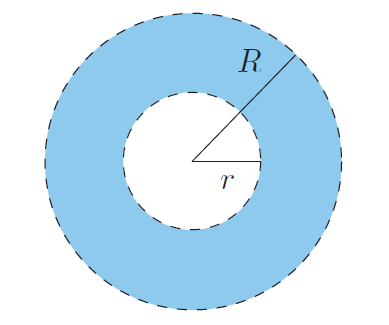
\includegraphics[width=0.3\textwidth]{./SaltChapter/fig-4-0-7}
\end{center}
%\caption{$\mathbb C$에 정의된 제곱급수의 수렴영역}
%\label{fig-4-0-3}
\end{figure*}

앞으로 다음을 살펴볼 예정이다.
\begin{itemize}
\item[(1)] 로랑 급수는 $z_0$ 중심의 
원환 $\{ z\in \mathbb C \,:\, r < |z-z_0| <R\}$에서 ``수렴''하는
복소해석함수가 된다.
\item[(2)] 역으로, $z_0$를 중심으로 하는 원환에 정의된 복소해석함수가
특이점을 원환의 안쪽 구멍에서만 갖는다면
함수는 원환에서 로랑급수를 갖는다. 예를 들어 모든 $z\in \mathbb C$에 대하여
\[
\exp z = 1 + \dfrac{z}{1!} + \dfrac{z^2}{2!} + \dfrac{z^3}{3!} + \cdots
\]
이고 $z\ne0$에 대한 ``로랑 급수 전개''는
\[
\exp \dfrac1z = 1 + \dfrac{1}{z} + \dfrac{1}{2!}\dfrac1{z^2} + \dfrac{1}{3!}\dfrac1{z^3} + \cdots.
\]
$\exp(1/z)$는 $\mathbb C\setminus \{0\}$에서 복소해석함수이다.
$\mathbb C\setminus \{0\}$는 원환의 퇴화된 모습으로
중심이 $0$이고 안쪽 반지름 $r=0$, 바깥쪽 반지름 $R=+\infty$인 경우다.
\end{itemize}

우선 $\Sum_{n\in \mathbb Z} c_n(z-z_0)^n$의 수렴에 대한 개념부터 만들자.

\begin{salt_definition} \label{def-4-3}
\[
\Sum_{n=1}^\infty c_{-n}(z-z_0)^n, \quad
\Sum_{n=0}^\infty c_{n}(z-z_0)^n
\]
이 모두 수렴하면, 
로랑 급수  $\Sum_{n\in \mathbb Z} c_n(z-z_0)^n$가 수렴한다.

$\Sum_{n\in \mathbb Z} c_n(z-z_0)^n$가 수렴하면, 다음과 같이 쓸 수 있고
\[
\Sum_{n\in \mathbb Z} c_n(z-z_0)^n
= \Sum_{n=1}^\infty c_{-n}(z-z_0)^n + \Sum_{n=0}^\infty c_{n}(z-z_0)^n
\]
는 로랑 급수의 합이라 부른다.
\end{salt_definition}

\begin{salt_example} \label{example-4-10}

\end{salt_example}






